\tikzset{
every node/.style={draw,text width=2cm},
style1/.style= {rectangle, rounded corners=2pt, thin,align=center,fill=green!30,text width=5cm},
style2/.style= {rectangle, rounded corners=6pt, thin,align=center,fill=green!60,yshift=-2cm,text width=2.5cm},
style3/.style= {rectangle,thin,align=left,fill=blue!20,yshift=-1cm,text width=2.5cm},
style4/.style= {draw=white,thin,align=center,fill=white}
}


\begin{figure}[ht!]
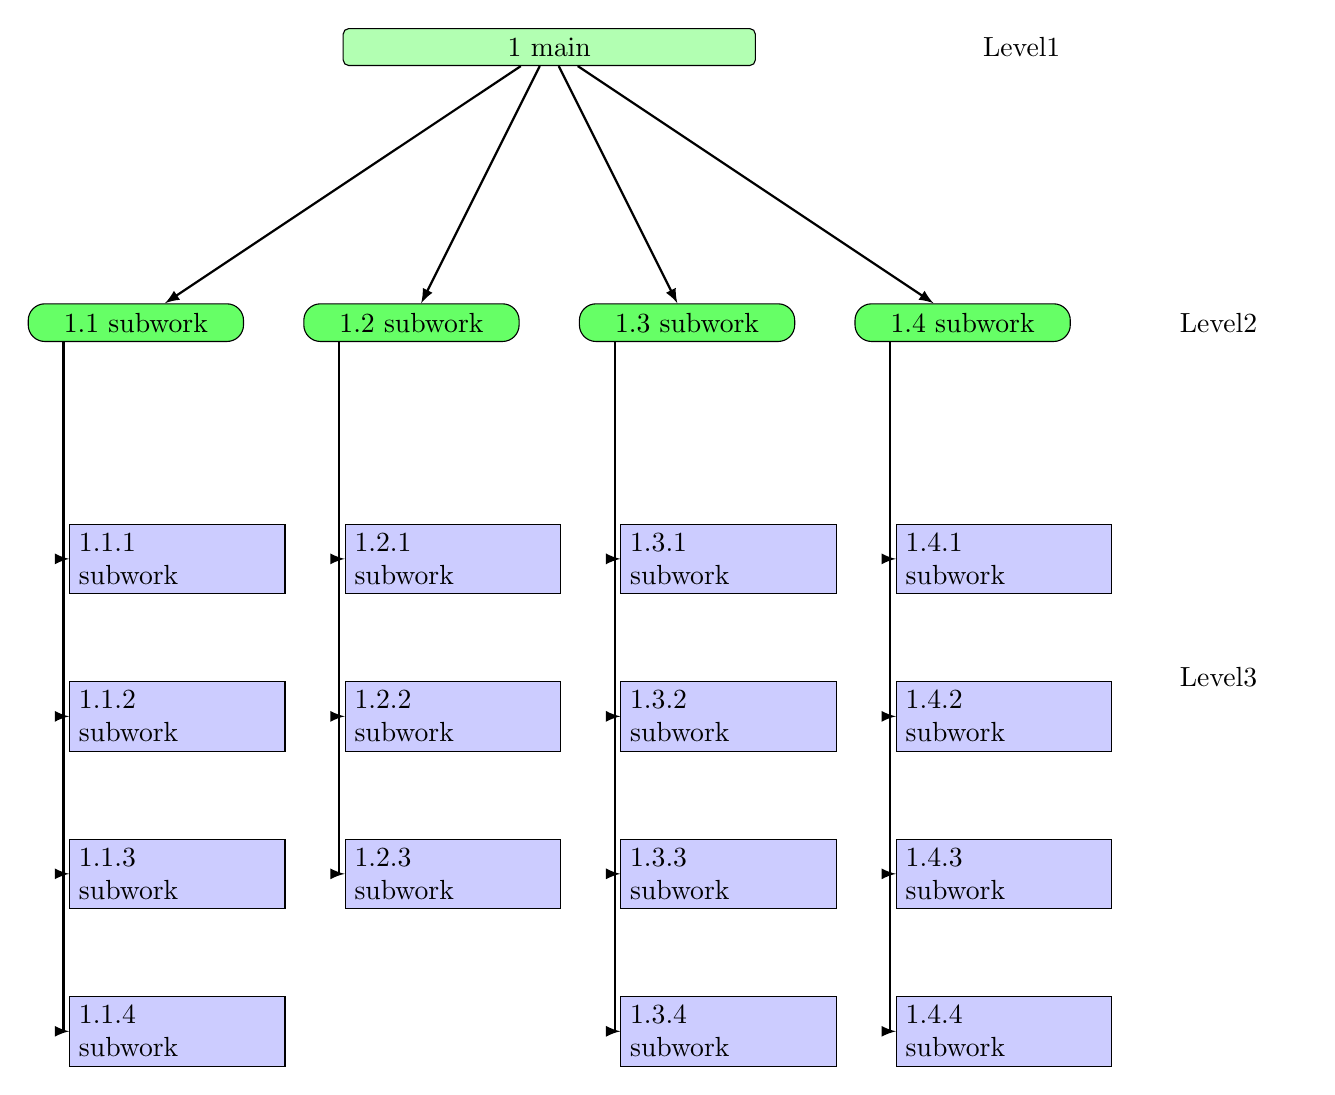
\begin{tikzpicture}[
remember picture,
level 1/.style={sibling distance=35mm},
edge from parent/.style={->,draw,thick},
>=latex]

% the initial tree ("root" and "text nodes")
\node[style1] {1 main}
child {node[style2] (c1) {1.1 subwork}}
child {node[style2] (c2) {1.2 subwork}}
child {node[style2] (c3) {1.3 subwork}}
child {node[style2] (c4) {1.4 subwork}};

% the nodes below each of the "text" nodes
\node [style3,below of = c1,xshift=15pt,yshift=-1cm] (c11) {1.1.1 \\ subwork};
\node [style3,below of = c11] (c12) {1.1.2\\subwork};
\node [style3,below of = c12] (c13) {1.1.3\\ subwork};
\node [style3,below of = c13] (c14) {1.1.4\\subwork};

\node [style3,below of = c2,xshift=15pt,yshift=-1cm] (c21) {1.2.1\\subwork};
\node [style3,below of = c21] (c22) {1.2.2\\subwork};
\node [style3,below of = c22] (c23) {1.2.3\\subwork};

\node [style3,below of = c3,xshift=15pt,yshift=-1cm] (c31) {1.3.1\\subwork};
\node [style3,below of = c31] (c32) {1.3.2\\subwork};
\node [style3,below of = c32] (c33) {1.3.3\\subwork};
\node [style3,below of = c33] (c34) {1.3.4\\subwork};

\node [style3,below of = c4,xshift=15pt,yshift=-1cm] (c41) {1.4.1\\subwork};
\node [style3,below of = c41] (c42) {1.4.2\\subwork};
\node [style3,below of = c42] (c43) {1.4.3\\subwork};
\node [style3,below of = c43] (c44) {1.4.4\\subwork};

\node[style4] at (6,0) {Level1};
\node[style4] at (8.5,-3.5) {Level2};
\node[style4] at (8.5,-8) {Level3};

% lines from each "text" node to every one of its "children"
\foreach \value in {1,2,3,4}
  \draw[thick,->] (c1.195) |- (c1\value.west);

\foreach \value in {1,...,3}
  \draw[thick,->] (c2.195) |- (c2\value.west);

\foreach \value in {1,...,4}
  \draw[thick,->] (c3.195) |- (c3\value.west);

\foreach \value in {1,...,4}
 \draw[thick,->] (c4.195) |- (c4\value.west);
\end{tikzpicture}
\caption{Work Breakdown Structure}
\label{fig:wbs}
\end{figure}
